\subsection{AMADA bending machine}
% Table for bending machine details
\begin{table}[h!]
    \centering
    \renewcommand{\arraystretch}{1.2} % Adjusts row height
    \small
    \begin{tabular}{ll}
        {\textbf{Description}} & {\textbf{Value}} \\
        \hline
        \textbf{Model} & HFP 50-20 \\
        \textbf{Manufacturer} & \hyperref[acro:AMADA]{AMADA} (France) \\
        \textbf{Year of manufacture} & 2005 \\
        \textbf{Drive} & Hydraulic press brake \\
        \textbf{Pressing capacity} & 500 kN \\
        \textbf{Working length} & 2090 mm \\
        \textbf{Distance between frames} & 1665 mm \\
        \textbf{\hyperref[acro:CNC]{CNC} control} & AMADA AMNC \hyperref[acro:3D]{3D}-graphic \\
        & with \hyperref[acro:TFT]{TFT} color screen \\
        \textbf{controlled axes} &  Y1/Y2; X1/X2; R1/R2; Z1/Z2 \\
        \textbf{Open height} & 470 mm \\
        \textbf{Stroke} & 200 mm \\
        \textbf{Bending Speed} & 10 mm/s \\
        \textbf{Approach Speed} & 100 mm/s \\
        \textbf{Return Speed} & 100 mm/s \\
        \textbf{Laser monitoring} & FIESSLER \\
        \textbf{Length x width x height} & 3458 mm x 2450 mm x 2450 mm \\
        \textbf{Weight} & 4850 kg \\ \hline
    \end{tabular}
    \caption{Bending Machine Technical Specifications (Source: \cite{bmspecifications})}
    \label{tab:machine_specifications}
\end{table}



\subsection{Kassow Robots: KR1410}

KR1410 is a 7-axis collaborative robotic arm from Kassow Robots. It has a reachability of 1400 mm which fits
satisfactory in the workcell. A seventh axis is particulary useful as it allows more freedom during trajectory planning
especially in close spaces.

The robotic arm comes with a robot controller and a teach pendant as shown in Figure \ref{fig:kassow-robot-parts} A robot controller is the main controlling unit for each \hyperref[acro:KR]{KR} manipulator.
Teach Pendant is used for programming the manipulator and also provides \hyperref[acro:UI]{UI} and safety controls.
KR1410 could be interfaced with ROS. KR provides packages to install through which KR messages transmission is set up.

\begin{figure}[h]
    \centering
    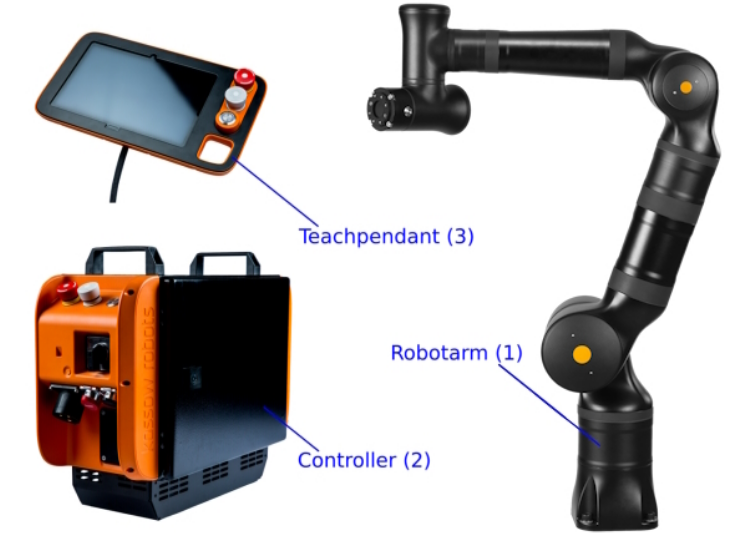
\includegraphics[width=0.5\textwidth]{figures/kassow-robot-parts.png}
    \caption{Functional parts of the KR collaborative robot (Source: \cite{kassow-manual})}
    \label{fig:kassow-robot-parts}
\end{figure}

\subsubsection{Function Description}
Function Description
\begin{enumerate}
    \item 
\end{enumerate}
The industrial robot arm is a robot system used for manufacturing. It is automated, programmable and
capable of moving within up to seven axes.
The robot is typically used for welding, painting, assembly, pick and place, packaging and labelling.
\begin{table}[h!]
    \centering
    \small
    \renewcommand{\arraystretch}{1.2} % Adjusts row height
    \begin{tabular}{ll}
        \textbf{Description} & \textbf{Value} \\ \hline
        Type & Collaborative \\
        Reach & 1400 mm in all directions\\
        Number of axis & 7-axis \\
        Operating temperature range & 0-45°C\\ 
        Weight & 38.0 kg \\ 
        AC Power connector & 1 Phase CEE \\ 
        Typical Power consumption & 400-1200W \\ 
        Supply voltage & 100-120 and 200-240 VAC (50/60hz) \\ 
        Supply current & 16A\\ 
        \hyperref[acro:IO]{IO} power supply & 24 VDC\\ 
        Max. joint speed  & 163/225 °/s\\ 
        Max. static force on \hyperref[acro:TFC]{TFC} (payload) & 10 kg\\ 
        Max. static torque on \hyperref[acro:TFC]{TFC} & 25 Nm\\ 
        Sound level & Below 70dB (A) \\ 
        Ingress protection & IP54 \\ 
        Joint ranges & Joint 1,3,5,6,7 +/- 360° \\
        & Joint 2,4 -70/+180° \\ 
        Footprint& $160 \times 160$ mm \\ 
        ROS Support & Available \\ \hline
    \end{tabular}
    \caption{KR1410 Technical Specifications (Source: \cite[page 31]{kassow-specification})}
    \end{table}

    \subsubsection{Increased Safety}

    Industrial Robotic Automation significantly enhances workplace safety. Robots, especially cobots like Kassow Robot's 7-axis version, are equipped with advanced safety features and mechanisms. 
    They can detect and avoid collisions with people or objects, reducing the risks associated with manual labour in potentially hazardous environments. This commitment to safety exemplifies the primary objective of robotic automation: to protect workers and streamline processes.

    \subsubsection{More Flexibility}
    Cobots, with their adaptable designs, represent the epitome of flexibility in industrial automation. 
    Unlike traditional fixed robots, the 7-axis from Kassow Robots can be quickly reprogrammed and adapted for different tasks. This agility makes them an invaluable asset for industries undergoing frequent changes or those with diverse product lines.

    \subsubsection{Cost-effective}
    Introducing Industrial Robotic Automation is a wise financial decision for businesses. Cobots, which offer a competitive price point compared to traditional industrial robots, provide significant returns on investment by improving efficiency, reducing waste, and minimizing production downtime. 
    The long-term savings, in terms of both time and money, underscore the economic benefits of integrating robotic automation into the production process.

    \subsubsection{Great Scalability}
    Industrial robots, especially cobots, are inherently scalable. Whether it's adjusting to a new product line or ramping up production volumes, Kassow Robot's 7-axis cobot can be swiftly recalibrated to meet evolving demands. 
    This ensures that industries can easily scale their operations without undergoing extensive overhauls or incurring excessive costs.

    \subsubsection*{Improved Quality}
    Quality assurance is a prominent benefit of Industrial Robotic Automation. Robots, with their precision and consistency, dramatically reduce the margin for errors in production. 
    Kassow Robot's 7-axis model ensures that each task—from welding to assembly—is executed with remarkable accuracy, leading to products of superior quality and consistency.

    \subsubsection*{Higher Productivity}

    Robotic automation directly translates to increased productivity. By automating repetitive and time-consuming tasks, cobots free human workers to concentrate on value-added activities. 
    In scenarios where cobots collaborate with human workers, the synergy often leads to faster production cycles, efficient workflows, and overall heightened productivity.

    
\subsection{VISOR\textsuperscript{\textregistered} Vision Sensor}
\label{sec:visor}
    According to \hyperref[acro:VISOR]{VISOR}\textsuperscript{\textregistered} \cite[page 22]{visor_user_manual} user manual, the \hyperref[acro:VISOR]{VISOR}\textsuperscript{\textregistered} vision sensor is an optical sensor and is used for the non-contact acquisition or identification of objects.
    The vision sensor features a number of different evaluation methods (detectors), with the specific methods
    depending on the specific model sensor. The product is designed for industrial use only. The \hyperref[acro:VISOR]{VISOR}\textsuperscript{\textregistered} vision sensor is a cost-effective alternative to conventional image processing systems.

    \hyperref[acro:VISOR]{VISOR}\textsuperscript{\textregistered} vision sensor is a suitable choice for the identification and classification of metal sheets for the automated bending process.
    These sensors enable precise detection and processing of features on sheets, which leads to the efficiency and accuracy of automated bending process.
    Special considerations need to be taken in complex industrial environments, where light reflections or changing extraneous light can distort evaluation results. For this reason, an external light source is used to protect against ambient light.

    \subsection{Robotic Camera}
    \label{subsec:robotic-camera}

    \subsection{Inspection Camera}
    \label{subsec:inspection-camera}